% Kapitel 'Betrachtungstransformationen'
\chapter{Betrachtungstransformationen}
\label{viewingtransformations}
Im vorigen Kapitel haben wir die verschiedenen Formen von Skalierung, Translation und Rotation behandelt, die für die Platzierung und Ausrichtung der einzelnen Modelle in der Szene, also für das Berechnen der World Matrix, nötig sind. Das Thema dieses Kapitel ist die Transformationen, die für den Übergang vom Weltkoordinatensystem in das Bildschirmkoordinatensystem verwendet werden.

\section{View Matrix}
\label{view}
In der 3D-Programmierung haben sich zwei praktische Arten eingebürgert, um die Ansicht auf die Szene festzulegen: Die Position des Betrachters kombiniert mit seiner Blickrichtung oder einem Punkt, den er anvisiert. Die View Matrix, die aus diesen Parametern berechnet wird, überführt das Weltkoordinatensystem in das Kamerakoordinatensystem, das seinen Ursprung im Auge des virtuellen Betrachters hat. Die $x$-Achse des neuen Systems zeigt dabei nach rechts, die $y$-Achse nach oben, und die $z$-Achse (in einem rechtshändigen System) gegen die Blickrichtung.

Im ersten Fall sind drei Vektoren gegeben: der Positionsvektor $\vec p$, der Richtungsvektor $\vec d$ und der Hochvektor $\vec u$. Die Bedeutung von $\vec p$ und $\vec u$ sollte klar sein, der Hochvektor ist nötig, um festzulegen, welche Richtung für den Betrachter \enquote{oben} ist. Alle Vektoren haben Einheitslänge, $\vec u$ steht senkrecht auf $\vec d$. Der dritte Basisvektor des neuen Koordinatensystems, der Rechtsvektor $\vec r$, lässt sich leicht über das Kreuzprodukt berechnen:
\begin{equation}
 \vec r = \vec d \times \vec u
\end{equation}

Im zweiten Fall ist neben $\vec p$ nur die Position des Ziels, $\vec t$, gegeben. Der Hochvektor muss aus dem Hochvektor $\vec u_w$ des Weltkoordinatensystems (normalerweise \textvec{0}{1}{0}) berechnet werden. In der Regel wird diese Darstellung in die erste Variante konvertiert, um dann daraus die Matrix zu berechnen. Dazu wird zunächst der normierte Richtungsvektor $\vec d$ berechnet, der von der Position der Kamera zum Ziel zeigt:
\begin{equation}
 \vec d = \frac{\vec t - \vec p}{\left| \vec t - \vec p \right|}
\end{equation}
Der Rechtsvektor muss senkrecht auf der zwischen Welt-Hochvektor und Richtungsvektor aufgespannten Ebene stehen. Er lässt sich daher über das Kreuzprodukt gewinnen:
\begin{equation}
 \vec r = \frac{\vec d \times \vec u_w}{\left| \vec d \times \vec u_w \right|}
\end{equation} 
Der Hochvektor berechnet sich nun als Kreuzprodukt aus Rechts- und Richtungsvektor
\begin{equation}
 \vec u = \vec r \times \vec d = \frac{\left( \vec d \times \vec u_w \right) \times \vec d}{\left| \left( \vec d \times \vec u_w \right) \times \vec d \right|},
\end{equation} 
was sich unter Zuhilfenahme der Grassmann-Identität zu dem schneller zu berechnenden Ausdruck
\begin{equation}
 \vec u = \frac{ \vec{u_w} - \left( \vec{d} \cdot \vec{u_w} \right) \cdot \vec{d} }{\left| \vec{u_w} - \left( \vec{d} \cdot \vec{u_w} \right) \cdot \vec{d} \right|}
\end{equation} 
vereinfachen lässt.

In beiden Fällen geht es nun darum, aus $\vec p$, $\vec d$, $\vec u$ und $\vec r$ die Transformationsmatrix zu bestimmen. Die Transformation in das Kamerakoordinatensystem kann in zwei Schritte aufgeteilt werden: Zuerst wird der Ursprung des Koordinatensystems in den Standpunkt der Kamera verschoben, dann werden die Achsen korrekt ausgerichtet.

Um den Ursprung in $\vec p$ zu verschieben, müssen alle Objekte um $-\vec p$ verschoben werden:
\begin{equation}
 M_{trans} = \begin{pmatrix}
  1 & 0 & 0 & -p_x \\
  0 & 1 & 0 & -p_y \\
  0 & 0 & 1 & -p_z \\
  0 & 0 & 0 & 1
 \end{pmatrix}
\end{equation}

Die Vektoren $-\vec d$, $\vec u$ und $\vec r$ sind ja die Basisvektoren des Kamarakoordinatensystems, die Matrix für den Rotationsteil kann also wie in Kapitel \ref{rotationbasevectors} beschrieben aufgestellt werden. Dabei ist zu beachten, dass die Rotation der Kamera ja rückgängig gemacht werden soll, die entstehende Matrix also invertiert werden muss:
\begin{equation}
 M_{rot} =
 \begin{pmatrix}
  r_x & u_x & -d_x & 0 \\
  r_y & u_y & -d_y & 0 \\
  r_z & u_z & -d_z & 0 \\
  0 & 0 & 0 & 1
 \end{pmatrix}^{-1} =
 \begin{pmatrix}
   r_x &  r_y &  r_z & 0 \\
   u_x &  u_y &  u_z & 0 \\
  -d_x & -d_y & -d_z & 0 \\
   0 & 0 & 0 & 1
 \end{pmatrix}
\end{equation}
% @clarify

Um die fertige View Matrix zu erhalten, müssen die beiden Matrizen nur noch multipliziert werden:
\begin{equation}
\begin{split}
 M_{view} &= M_{rot} \cdot M_{trans} \\
 &=
 \begin{pmatrix}
   r_x &  r_y &  r_z & 0 \\
   u_x &  u_y &  u_z & 0 \\
  -d_x & -d_y & -d_z & 0 \\
   0 & 0 & 0 & 1
 \end{pmatrix} \cdot 
 \begin{pmatrix}
  1 & 0 & 0 & -p_x \\
  0 & 1 & 0 & -p_y \\
  0 & 0 & 1 & -p_z \\
  0 & 0 & 0 & 1
 \end{pmatrix} \\
 M_{view} &=
 \begin{pmatrix}
   r_x &  r_y &  r_z & -\vec r \cdot \vec p \\
   u_x &  u_y &  u_z & -\vec u \cdot \vec p \\
  -d_x & -d_y & -d_z & \vec d \cdot \vec p \\
   0 & 0 & 0 & 1
 \end{pmatrix}
\end{split}
\end{equation}

\section{Projection Matrix}
\label{projection}
Die Positionen aller Vertices liegen nach der Transformation durch die View Matrix also im lokalen Koordinatensystem der Kamera vor. Um aus den dreidimensionalen Koordinaten im Raum die zweidimensionalen Bildschirmkoodinaten zu erhalten, müssen sie in irgendeiner Form projiziert werden. Für diese Projektion gibt es je nach Anwendungsgebiet viele Möglichkeiten, darunter auch eher exotische wie die Projektion auf einen Zylindermantel oder krummlinige Projektionen, um Linseneffekte zu simulieren. Aber selbst wenn man sich auf den einfachsten Fall, die Projektion auf eine Ebene, beschränkt, gibt es noch immer zahlreiche Unterarten. \vgls{script:spain}{115-117}

Ich werde mich hier auf die bei Weitem am häufigsten verwendete Art beschränken, die \emph{Zentralprojektion}. Hier wird ein Punkt projiziert, indem man die Linie durch den Punkt und ein gemeinsames Projektionszentrum mit der Bildebene schneidet. Geraden bleiben dabei auch in der Abbildung Geraden, im dreidimensionalen Raum parallele Kanten schneiden sich in einem gemeinsamen Fluchtpunkt. Die Zentralprojektion ist der Abbildung durch das menschliche Auge sehr ähnlich und ermöglicht somit natürlich wirkende Bilder. \vglr{wiki:zentralprojektion}

% Drawing 'Zentralprojektion'

Das \emph{Sichtvolumen} der Zentralprojektion wird also grundsätzlich von den Strahlen durch den Augpunkt und die Ecken des Sichtfensters aufgespannt, ist also eine unendliche rechteckige Pyramide mit der Spitze im Augpunkt \textvec{0}{0}{0}. Die Projektion wird normalerweise durch zwei Parameter charakterisiert: den vertikalen Öffnungswinkel des Sichtvolumens, $\varphi$, und das Seitenverhältnis des Sichtfensters (also im Normalfall des Bildschirmes), $\frac{W}{H} = r$. Wir werden hier nur die normalerweise verwendete \emph{symmetrische Zentralprojektion} behandeln, bei der der Augpunkt in das Zentrum des Bildes projiziert wird.

Wie bereits in Kapitel \ref{coordinatesystems} erwähnt, besteht die Aufgabe der Projection Matrix darin, dieses Sichtvolumen in das \emph{kanonische Sichtvolumen} zu überführen, wonach die Geometrie wieder für alle Arten von Projektion gleich behandelt wird. Auch für das kanonische Sichtvolumen gibt es wieder unterschiedliche Konventionen, wir werden hier die DirectX-Variante behandeln, einen Quader zwischen den Punkten \textvec{-1}{-1}{0} und \textvec{1}{1}{1}. \vglr{directx:transformationpipeline}

\begin{wrapfigure}{R}{0.5\textwidth}
  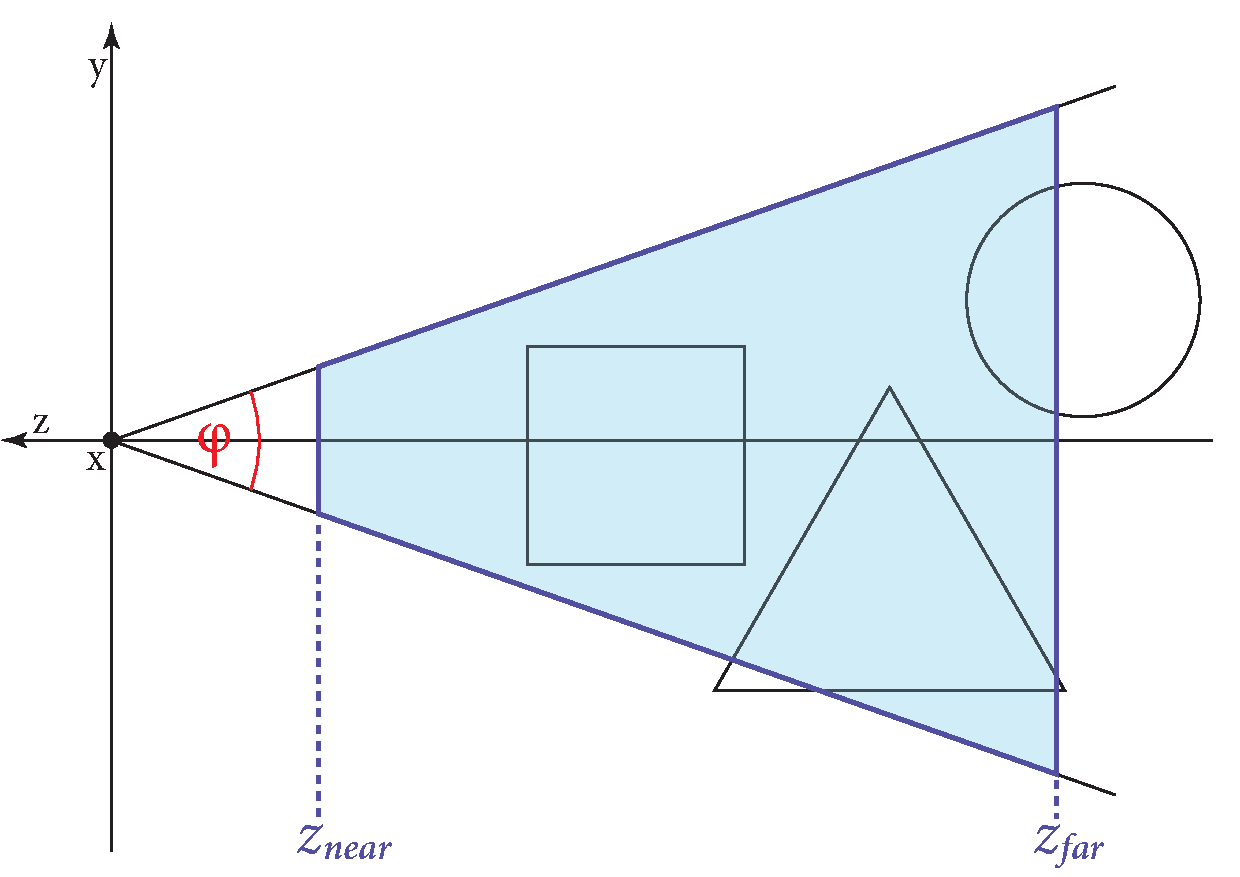
\includegraphics[width=0.49\textwidth]{clippingplanes}
  \caption{Near- und Far Clipping Plane.}
  \label{image:clippingplanes}
\end{wrapfigure}

Für die Transformation muss das Sichtvolumen aber zuerst begrenzt werden, da sonst verschiedene grundsätzliche und numerische Probleme entstehen werden\footnote{Beispielsweise würden Punkte, die exakt im Augpunkt liegen, Probleme verursachen und sehr weit entfernte Objekte würden im Hinblick auf die begrenzte Rechengenauigkeit problematisch sein.}. Das geschieht mit zwei zur $z$-Achse senkrechten Ebenen, der \emph{Near Clipping Plane} und der \emph{Far Clipping Plane} (von engl. \emph{to clip}, \enquote{abschneiden}). Das entstehende Volumen ist ein Pyramidenstumpf, in der 3D-Grafik meist mit dem englischen Begriff \emph{Frustum} bezeichnet.

Besonders wichtig ist die Begrenzung des Sichtvolumens für die auf die Projektion folgende Sichtbarkeitsbestimmung, da hier wie auch sonst in Computerprogrammen mit einer beschränkten Genaugkeit gerechnet wird. Ist der Abstand von Near und Far Clipping Plane zu groß, macht sich die begrenzte Genauigkeit bemerkbar und es kommt zu einem als \emph{Z-Fighting} bekannten Phänomen, bei dem auf nicht-deterministische Weise abwechselnd verschiedene Pixel von Polygonen in einer ähnlichen Tiefe im Vordergrund gezeichnet werden.

Zur Herleitung der Projection Matrix für die Zentralprojektion transformieren wir das Sichtvolumen zunächst einmal so, dass der horizontale und der vertikale Öffnungswinkel $90^\circ$ betragen ($\varphi = 90^\circ$ und $r = 1$). Dazu ist eine Skalierung entlang der $x$- und der $y$-Achse nötig: Wie sich aus Abbildung \ref{image:clippingplanes} und \ref{image:rightangledvolume} leicht erkennen lässt, wächst die $y$-Koordinate der oberen und unteren Begrenzung des Frustums bei steigender $z$-Koordinate mit dem Faktor $\pm \tan\frac{\varphi}{2}$, im transformierten Frustum aber mit dem Faktor $\pm 1$. Die $x$-Koordinate der linken und der rechten Grenze verhalten sich bis auf den Faktor für das Seitenverhältnis genauso. Das Sichtvolumen muss also um den Faktor $1 : (\tan\frac{\varphi}{2})$ in $y$-Richtung und $1 : (\tan\frac{\varphi}{2} \cdot r)$ in $x$-Richtung skaliert werden.

\begin{wrapfigure}{R}{0.35\textwidth}
  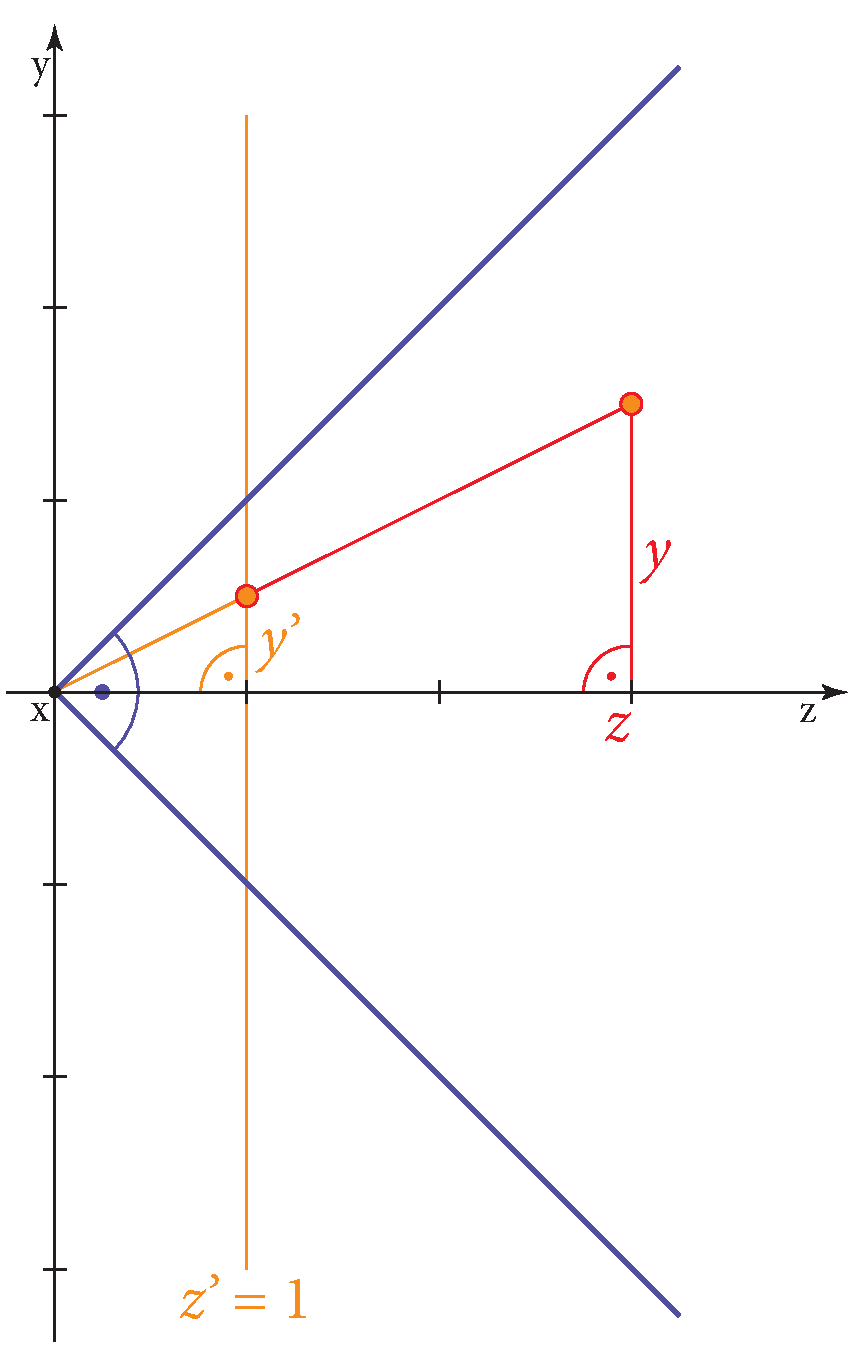
\includegraphics[width=0.34\textwidth]{rightangledvolume}
  \caption{Rechtwinkliges Sichtvolumen mit Projektion auf die Ebene $z=1$.}
  \label{image:rightangledvolume}
\end{wrapfigure}

Daneben spiegeln wir das Koordinatensystem an der $xy$-Ebene, um ein intuitiveres Arbeiten zu ermöglichen -- mit steigendem Abstand von der Kamera wächst nun auch die $z$-Koordinate. Für diesen ersten Schritt ergibt sich also die Matrix
\begin{equation}
 P_1 = \begin{pmatrix}
  \frac{1}{r \cdot \tan\frac{\varphi}{2}} & 0 & 0 & 0 \\
  0 & \frac{1}{\tan\frac{\varphi}{2}} & 0 & 0 \\
  0 & 0 & -1 & 0 \\
  0 & 0 & 0 & 1
 \end{pmatrix}.
\end{equation}

Danach werden die Punkte auf die Ebene $z=1$ projiziert. Wie aus Abbildung \ref{image:rightangledvolume} ersichtlich (ähnliche Dreiecke), gilt der Zusammenhang
\begin{equation}
 \frac{x'}{1} = \frac{x}{z}
\end{equation}
und analog für die $y$-Koordinate
\begin{equation}
 \frac{y'}{1} = \frac{y}{z}.
\end{equation}
Um die Projektion durchzuführen, müssen die $x$- und die $y$-Koordinate also durch die $z$-Koordinate dividiert werden. Um dies in eine Matrix zu verpacken, machen wir uns die homogenen Koordinaten zu Nutze, genauer die Konvention, dass der Vektor nachher durch Division durch $w$ wieder auf $w=1$ gebracht wird. Die Matrix braucht also einfach nur $w' = z$ zu setzen
\begin{equation}
 \begin{pmatrix}
  1 & 0 & 0 & 0 \\
  0 & 1 & 0 & 0 \\
  0 & 0 & 1 & 0 \\
  0 & 0 & 1 & 0
 \end{pmatrix}.
\end{equation}
Nach der Transformation mit dieser Matrix hat ein Vektor die Koordinaten \textvech{x}{y}{z}{z}, nach der homogenen Division also \textvec{\frac{x}{z}}{\frac{y}{z}}{1}.

Für die Projektion reicht diese Transformation an sich, und wie man leicht nachprüfen kann, befinden sich die $x$- und $y$-Koordinaten alle Punkte im Sichtvolumen jetzt zwischen $-1$ und $1$, wie es für das kanonische Sichtvolumen erforderlich ist. Allerdings ist durch die Projektion auch $z'$ für alle Punkte $1$, ist also unabhängig von $z$. Um später beim Zeichnen der Dreiecke die Sichtbarkeit korrekt bestimmen zu können, muss $z'$ aber mit wachsender Tiefe monoton steigen, die $z$-Reihenfolge der Punkte muss also erhalten bleiben. Um diese Bedingung zu erfüllen, werden zwei zusätzliche Parameter, $a$ und $b$, eingeführt:
\begin{equation}
 \begin{pmatrix}
  1 & 0 & 0 & 0 \\
  0 & 1 & 0 & 0 \\
  0 & 0 & a & b \\
  0 & 0 & 1 & 0
 \end{pmatrix}.
\end{equation}

Nach der Transformation und der homogenen Division ergibt sich mit dieser Matrix
\begin{equation}
 z' = \frac{a \cdot z + b}{z}.
\end{equation}

Nun müssen nur noch passende Werte für $a$ und $b$ gefunden werden. Aus der Definition des kanonischen Sichtvolumens folgen ja die Bedingungen, dass ein Punkt auf der Near Clipping Plane auf $z'=0$, und ein Punkt auf der Far Clipping Plane auf $z'=1$ abgebildet wird. Aus diesen Bedingungen ergibt sich also ein lineares Gleichungssystem mit zwei Variablen
\begin{equation}
\begin{split}
 0 = \frac{a \cdot z_\mathrm{near} + b}{z_\mathrm{near}} \\
 1 = \frac{a \cdot z_\mathrm{far} + b}{z_\mathrm{far}},
\end{split}
\end{equation}
welches sich einfach zu
\begin{equation}
\begin{split}
 a = \frac{z_\mathrm{far}}{z_\mathrm{far}-z_\mathrm{near}} \\
 b = -z_\mathrm{near} \cdot a = -\frac{z_\mathrm{far} \cdot z_\mathrm{near}}{z_\mathrm{far}-z_\mathrm{near}},
\end{split} 
\end{equation}
auflösen lässt. \vglr{perspectiveprojectionmatrix}

Für die Projektion des rechtwinkligen Sichtvolumens ergibt sich also die Matrix
\begin{equation}
 P_2 = \begin{pmatrix}
  1 & 0 & 0 & 0 \\
  0 & 1 & 0 & 0 \\
  0 & 0 & \frac{z_\mathrm{far}}{z_\mathrm{far}-z_\mathrm{near}} & -\frac{z_\mathrm{far} \cdot z_\mathrm{near}}{z_\mathrm{far}-z_\mathrm{near}} \\
  0 & 0 & 1 & 0
 \end{pmatrix}.
\end{equation}

Kombiniert man die beiden Matrizen durch Multiplikation, erhält man die \emph{Projection Matrix für die Zentralprojektion}:
\begin{equation}
\begin{split}
 M_{proj} = P_2 \cdot P_1 &= 
 \begin{pmatrix}
  \frac{1}{r \cdot \tan\frac{\varphi}{2}} & 0 & 0 & 0 \\
  0 & \frac{1}{\tan\frac{\varphi}{2}} & 0 & 0 \\
  0 & 0 & -\frac{z_\mathrm{far}}{z_\mathrm{far}-z_\mathrm{near}} & -\frac{z_\mathrm{far} \cdot z_\mathrm{near}}{z_\mathrm{far}-z_\mathrm{near}} \\
  0 & 0 & -1 & 0
 \end{pmatrix} \\
 &= 
 \begin{pmatrix}
  \frac{1}{r \cdot \tan\frac{\varphi}{2}} & 0 & 0 & 0 \\
  0 & \frac{1}{\tan\frac{\varphi}{2}} & 0 & 0 \\
  0 & 0 & \frac{z_\mathrm{far}}{z_\mathrm{near}-z_\mathrm{far}} & \frac{z_\mathrm{near} \cdot z_\mathrm{far}}{z_\mathrm{near}-z_\mathrm{far}} \\
  0 & 0 & -1 & 0
 \end{pmatrix}
\end{split}
\end{equation}

Nach der Transformation mit dieser Matrix befinden sich alle theoretisch sichtbaren Vertices im kanonischen Sichtvolumen, der Schritt der Projektion ist also abgeschlossen. Wie in Kapitel \ref{rendering} beschrieben, folgt nun das das \emph{Clipping}. In diesem Schritt wird die darzustellende Geometrie so abgeschnitten, dass sie nicht über das kanonische Sichtvolumen hinausragt. Hier gibt es bei der Behandlung eines Dreiecks grundsätzlich drei Möglichkeiten: Erstens kann es vollständig innerhalb des Sichtvolumens liegen, in diesem Fall bleibt es natürlich unverändert. Zweitens kann es vollständig außerhalb des Sichtvolumens liegen, es wird dann verworfen. Drittens kann es aber auch von einer oder mehreren der Begrenzungsflächen geschnitten werden. In diesem Fall wird das Dreieck verworfen und es werden neue Dreiecke generiert, welche die Fläche des Dreiecks, die innerhalb des Sichtvolumens liegt, ausfüllen.

Die $x$- und $y$-Koordinaten aller Vertices befinden sich nach dem Clipping also im Bereich $\left[ -1; 1 \right]$. Sie müssen dann nur noch in den Wertebereich des Ausgabemediums gebracht werden. Wenn ein typischer Bildschirm im $4:3$-Format ganz ausgefüllt werden soll, könnte dies beispielsweise der Bereich $\left[ 0; 1279 \right]$ horizontal und $\left[ 0; 959 \right]$ vertikal sein\footnote{Dies entspricht einer Bildschirmauflösung von $1280 \times 960$ -- in der Informatik wird fast immer $0$ als Index für das erste Element verwendet.}. Dieser Schritt wird als \emph{Viewport Transformation} bezeichnet und besteht im Normalfall aus einer Translation und einer Skalierung. Dabei ist zu berücksichtigen, dass die Werte in $y$-Richtung in allen vorherigen Koordinatensystemen nach oben wachsen, die $y$-Achse am Bildschirm aber nach unten zeigt. Es ist also eine Spiegelung an der $xz$-Ebene erforderlich.